\chapter{In-depth component description}

\section{Communicating with Channels}
\label{sec:channel}

\texttt{Channel} is an interface for performing I/O operations. It represents
the principal abstraction used by the middleware to communicate with hardware
devices and external software services.

\lstset{language=Java}
\begin{lstlisting}[float,caption=The Channel interface,label={lst:channel}]
public interface Channel {

	public String getId();
	
	public IOTask submit(IORequest request, IOHandler handler)
			throws ChannelException;
	
	public void setAsyncIOHandler(IOHandler handler)
			throws IllegalStateException;
			
	public boolean isClosed();
	
	public void close();
			
}
\end{lstlisting}

The \texttt{Channel} interface is not tied to any specific technology or
communication stack; as a result of this design choice, a wide variety of data
management tasks, including but not limited to, networking, file handling, and
automatic data generation can be implemented as \texttt{Channel}s.

The current Middleware architecture encourages the creation of several highly
specialized \texttt{Channel}s, which are usually developed around third-party
communication libraries. \texttt{HTTPChannel}, a \texttt{Channel} providing
support for HTTP communications, is an excellent example of the advantages of
this design strategy. Implemented as a simple wrapper around Apache's HTTP
Components toolkit, its development only required a basic understanding of the
HTTP protocol; yet \texttt{HTTPChannel} is a fully compliant HTTP/1.1 client
(see section~\ref{sec:channel.implementations} for additional details).

Upon instantiation, \texttt{Channel}s are open and ready to be used. They may
be optionally closed to relinquish unused resources by invoking the
\texttt{close()} method. Once closed, a \texttt{Channel} cannot be re-opened,
and every subsequent attempt to perform an I/O operation will fail causing a
\texttt{ChannelException} to be thrown. The current state of a \texttt{Channel}
can be probed through its \texttt{isClosed()} method.

Bytes sent or received with a \texttt{Channel} are encapsulated in a
\texttt{Payload} object. As shown in listing~\ref{lst:payload}, the
\texttt{Payload} interface allows all Middleware components to handle different
data types with a common set of methods, regardless of their individual
encoding.  \texttt{Payload}s will be the subject of further discussion in
section~\ref{sec:components.mapper}

\lstset{language=Java}
\begin{lstlisting}[float,caption=The Payload interface,label={lst:payload}]
public interface Payload {

	public Charset getCharset();

	public InputStream asInputStream();

	public ByteBuffer asByteBuffer();

	public String asString();

}
\end{lstlisting}

All user-initiated I/O operations begin with an invocation of the
\texttt{Channel.submit()} method. As can be seen in listing~\ref{lst:channel},
\texttt{submit()} is a direct implementation of the asynchronous interaction
paradigm introduced in section~\ref{sec:newmiddleware.async}. The emphasis on
asynchronous execution is underscored by the absence of blocking operations in
the \texttt{Channel} interface. This aspect is of paramount importance for the
entire Middleware design, as implementing a truly asynchronous system would
prove impossible if such feature were not provided by its core data access
layer.


\subsection{Instantiating new Channels}

\texttt{Channel}s are created by means of the \texttt{ChannelFactory}
interface, a reification of the Factory design pattern that allows polymorphic
instantiation of new object classes.

By using a Factory instantiation model, the choice of a particular
\texttt{Channel} implementation can be postponed from compile time to run time.
This technique allows the Middleware to dynamically adapt in response to
environment changes, and to support extension through the addition of new
user-defined \texttt{Channel}s. For further information regarding the Factory
pattern and its other uses inside the PerLa Middleware, refer to
section~\ref{sec:newmiddleware.factory}.

All the information required to create a new \texttt{Channel} is stored inside
a \texttt{ChannelDescriptor}. As shown in listing~\ref{lst:channelFactory},
this configuration object is the only parameter required to correctly invoke
the \texttt{createChannel()} method.

\lstset{language=Java}
\begin{lstlisting}[float,caption=The ChannelFactory
interface,label={lst:channelFactory}]
public interface ChannelFactory {

	public Class<? extends ChannelDescriptor>
			acceptedChannelDescriptorClass();

	public Channel createChannel(ChannelDescriptor descriptor)
			throws InvalidDeviceDescriptorException;

}
\end{lstlisting}

\begin{figure}[h!]
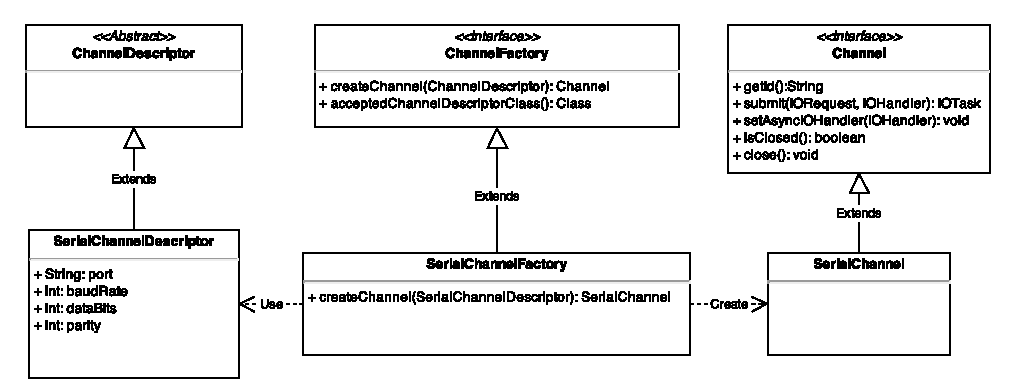
\includegraphics[width=\textwidth]{imgs/channel_factory.pdf}
\caption{Class diagram of the Channel layer}
\end{figure}

Each \texttt{ChannelFactory} is tied to a specific communication technology;
therefore, it can only accept a single class of \texttt{ChannelDescriptor}
objects. For example, the \texttt{HTTPChannelFactory} parses
\texttt{HTTPChannelDescriptor}s and creates \texttt{HTTPChannel}s, whereas an
hypothetical \texttt{SerialChannelFactory} would consume
\texttt{SerialChannelDescriptor}s to create \texttt{SerialChannel}s. Failure to
provide a suitable \texttt{ChannelDescriptor} object will cause the
\texttt{createChannel()} method to throw an
\texttt{InvalidDeviceDescriptorException}.

The \texttt{acceptedChannelDescriptorClass()} method can be used to dynamically
discover which \texttt{ChannelDescriptor} type is supported by a specific
\texttt{ChannelFactory}. This method is the fulcrum of the \texttt{Channel}
Plugin System, as it allows the Middleware to invoke the most appropriate
\texttt{ChannelFactory} using only information available at runtime.

\begin{figure}[!hbt]
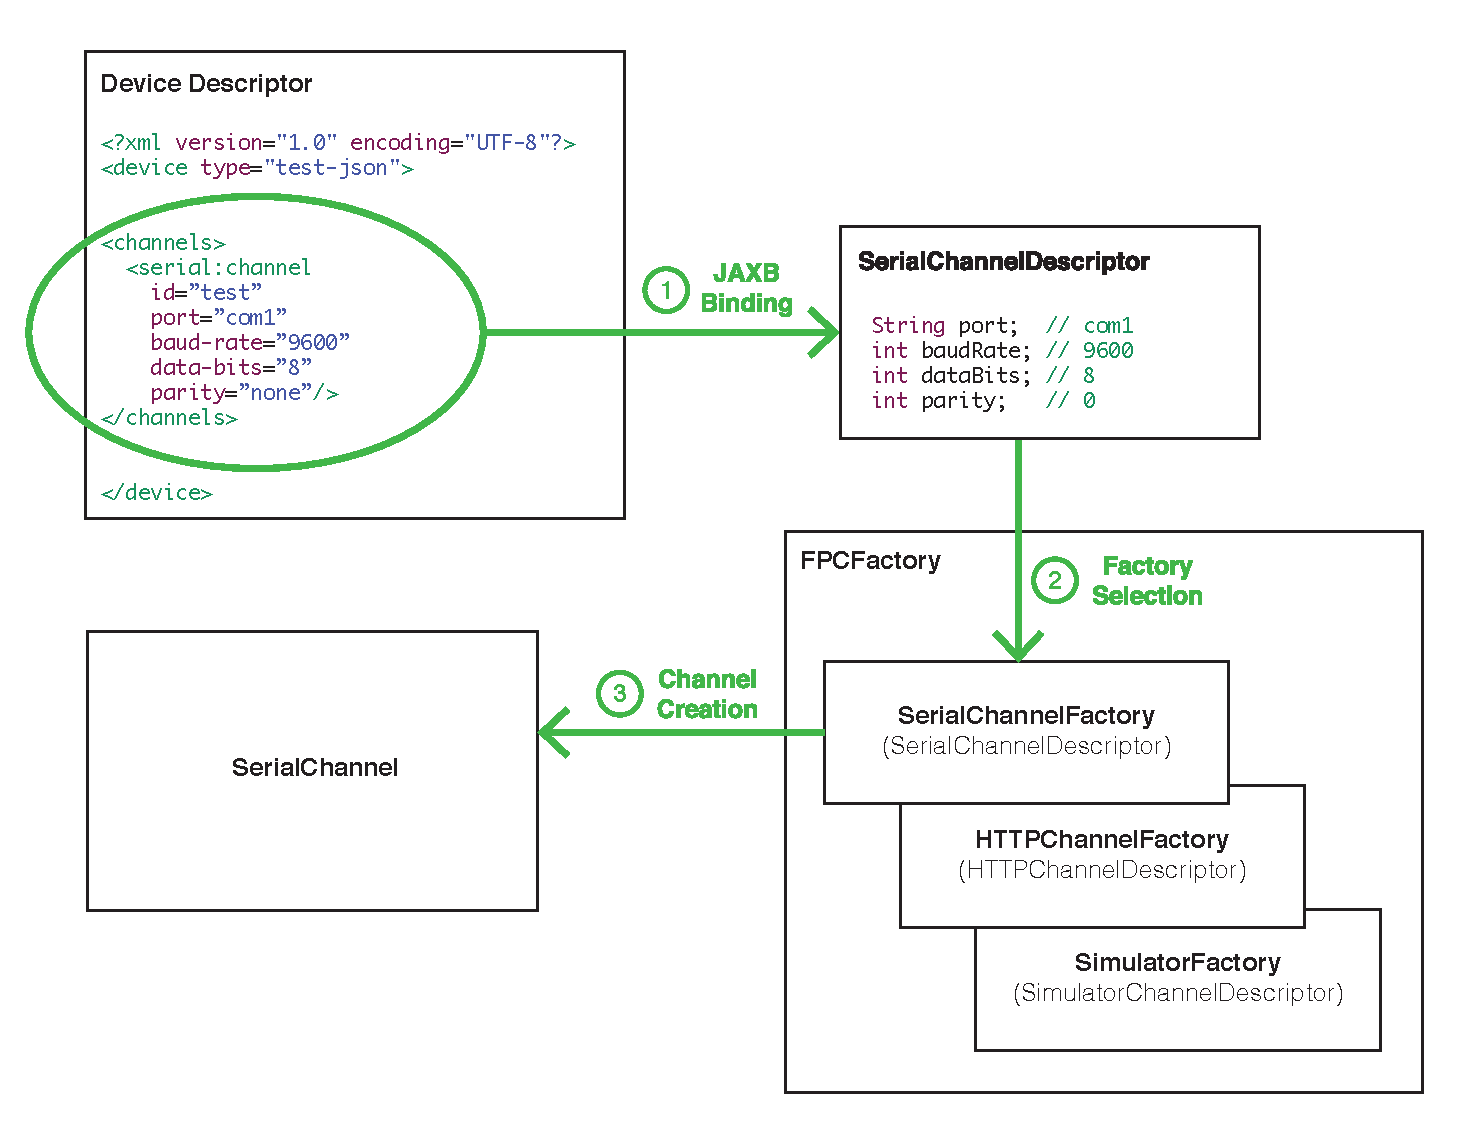
\includegraphics[width=\textwidth]{imgs/channel_creation_process.pdf}
\caption{The Channel creation process}
\label{fig:channel.creation}
{
\begin{figurenote}
This figure illustrates the \texttt{Channel} creation process executed by the
Middleware upon reception of a new Device Descriptor.  \begin{enumerate}
  \itemsep0em
  \item JAXB binds the XML Device Descriptor to an apropriate
\texttt{ChannelDescriptor} object using namespace information \item A suitable
\texttt{ChannelFactory} is selected at runtime using the
\texttt{acceptedChannelDescriptorClass()} method
  \item The information contained in the \texttt{SerialChannelDescriptor} is
used to create a new \texttt{SerialChannel} \end{enumerate}
\end{figurenote}
}
\end{figure}

\texttt{ChannelDescriptor} objects are automatically created by the
Middleware using the information contained in the Device Descriptor XML files.
This binding process is performed by the JAXB library, which is also
responsible for instantiating the correct \texttt{ChannelDescriptor} class
using XML Namespace information. Figure~\ref{fig:channel.creation} illustrates
this technique, and ties it together with the other operations described in
this section.

It is important to note that a single JVM instance running the PerLa Middleware
may host several \texttt{Channel} objects of the same type, at the same time.
Several devices can use the same communication technology, and the
\texttt{ChannelFactory} may determine that it's best to create an individual
\texttt{Channel} for each one of them. This behaviour is fostered by the new
\texttt{ChannelFactory} architecture, and is considered idiomatic design;
hence, it would not be uncommon to implement the hypothetical
\texttt{SerialChannelFactory} introduced in the previous paragraphs so that
every serial port is handled by a different \texttt{SerialChannel} instance.


\subsection{IORequest management}

\texttt{IORequest} is the base object interface employed to interact with a
sensing node connected to the Middleware. It contains two types of information:
the payload to be transferred, and \texttt{Channel}-dependent data needed for a
correct communication with the endpoint device.

\lstset{language=Java}
\begin{lstlisting}[float,floatplacement=!hbt,caption=The IORequest
interface,label={lst:iorequest}]
public interface IORequest {

	public String getId();

	public void setParameter(String name, Payload payload);
	
}
\end{lstlisting}

Every \texttt{Channel} imlementation is bundled with its own custom
\texttt{IORequest} class. Following up on previous examples, the
\texttt{HTTPChannel} package contains a \texttt{HTTPIORequest} object, whereas
the fictitious \texttt{SerialChannel} would be supplied with a
\texttt{SerialIORequest} class of request objects. This additional level of
indirection is necessary since different communication technologies require
different settings to establish end-to-end connectivity; therefore, a universal
\texttt{IORequest} object would soon prove to be a limiting factor for the
extension of the Middleware.

As shown in listing~\ref{lst:iorequest}, payload data can be set in an
\texttt{IORequest} by means of the \texttt{setParameter()} method.
\texttt{Payload}s are addressed by name, and a single \texttt{IORequest}
implementation may support several at once. The exact set of \texttt{Payload}
parameters accepted by an \texttt{IORequest} class depends on the design of its
matching \texttt{Channel}; for example, the \texttt{HTTPChannel}
implementation supports three: an `entity' payload (request body), a `query'
payload (an URL-encoded string), and a `path' payload (a path component used to
identify a single resource accessible from the base URL).

\texttt{IORequest}s are disposable objects; they are created, submitted to a
\texttt{Channel}, and garbage collected once the communication is over.
Creation is performed by means of a factory interface dubbed
\texttt{IORequestBuilder}, which allows the Middleware to build new copies of
an \texttt{IORequest} from a fixed template. It is important to note that
request objects built using this technique do not contain \texttt{Payload}
parameters; these are to be added manually before subbmitting the
\texttt{IORequest} to a \texttt{Channel}.

Besides \texttt{IORequest} creation, the \texttt{IORequestBuilder} interface
can be used to dynamically discover which \texttt{Payload} parameters are
supported by an \texttt{IORequest}. This functionality, exposed through the
\texttt{getParameterList()} method, is a crucial component of the Middleware
Plugin System, as it allows \texttt{Script} instructions to determine whether
an \texttt{IORequest} was populated with all the necessary \texttt{Payload}
parameters or not. This concept will be the subject of further analysis in
section~\ref{sec:components.script}.

A single device connected to the PerLa Middleware is generally managed using
several \texttt{IORequestBuilder}s, any one of which is responsible for
creating a request object suitable to control a single aspect of
the interaction with the endpoint. The main advantage brought by this
templating mechanism is that \texttt{Channel}-related configuration settings
are only specified once, hence the same \texttt{IORequest} structure can be
reused multiple times to transport different payload information.

\lstset{language=Java}
\begin{lstlisting}[float,floatplacement=!hbt,caption=The IORequestBuilder
interface,label={lst:iorequestbuilder}]
public interface IORequestBuilder {

	public String getRequestId();

	public IORequest create();

	public abstract List<IORequestParameter> getParameterList();

	public static class IORequestParameter {

		public String getName() {
			return name;
		}

		public boolean isMandatory() {
			return mandatory;
		}

	}
}
\end{lstlisting}

REST APIs are an excellent use case to demonstrate the aforementioned concept,
as every operation on a RESTful resource can be easily abstracted using an
appropriately configured request builder. By using
\texttt{HTTPIORequestBuilder} objects, HTTP protocol information (base URL,
method, header, \ldots) are specified one single time only for
every REST endpoint. Once this step is done, the API can be invoked just by
building new \texttt{IORequest}s and submitting them to a \texttt{HTTPChannel}.

\begin{figure}[!hbt]
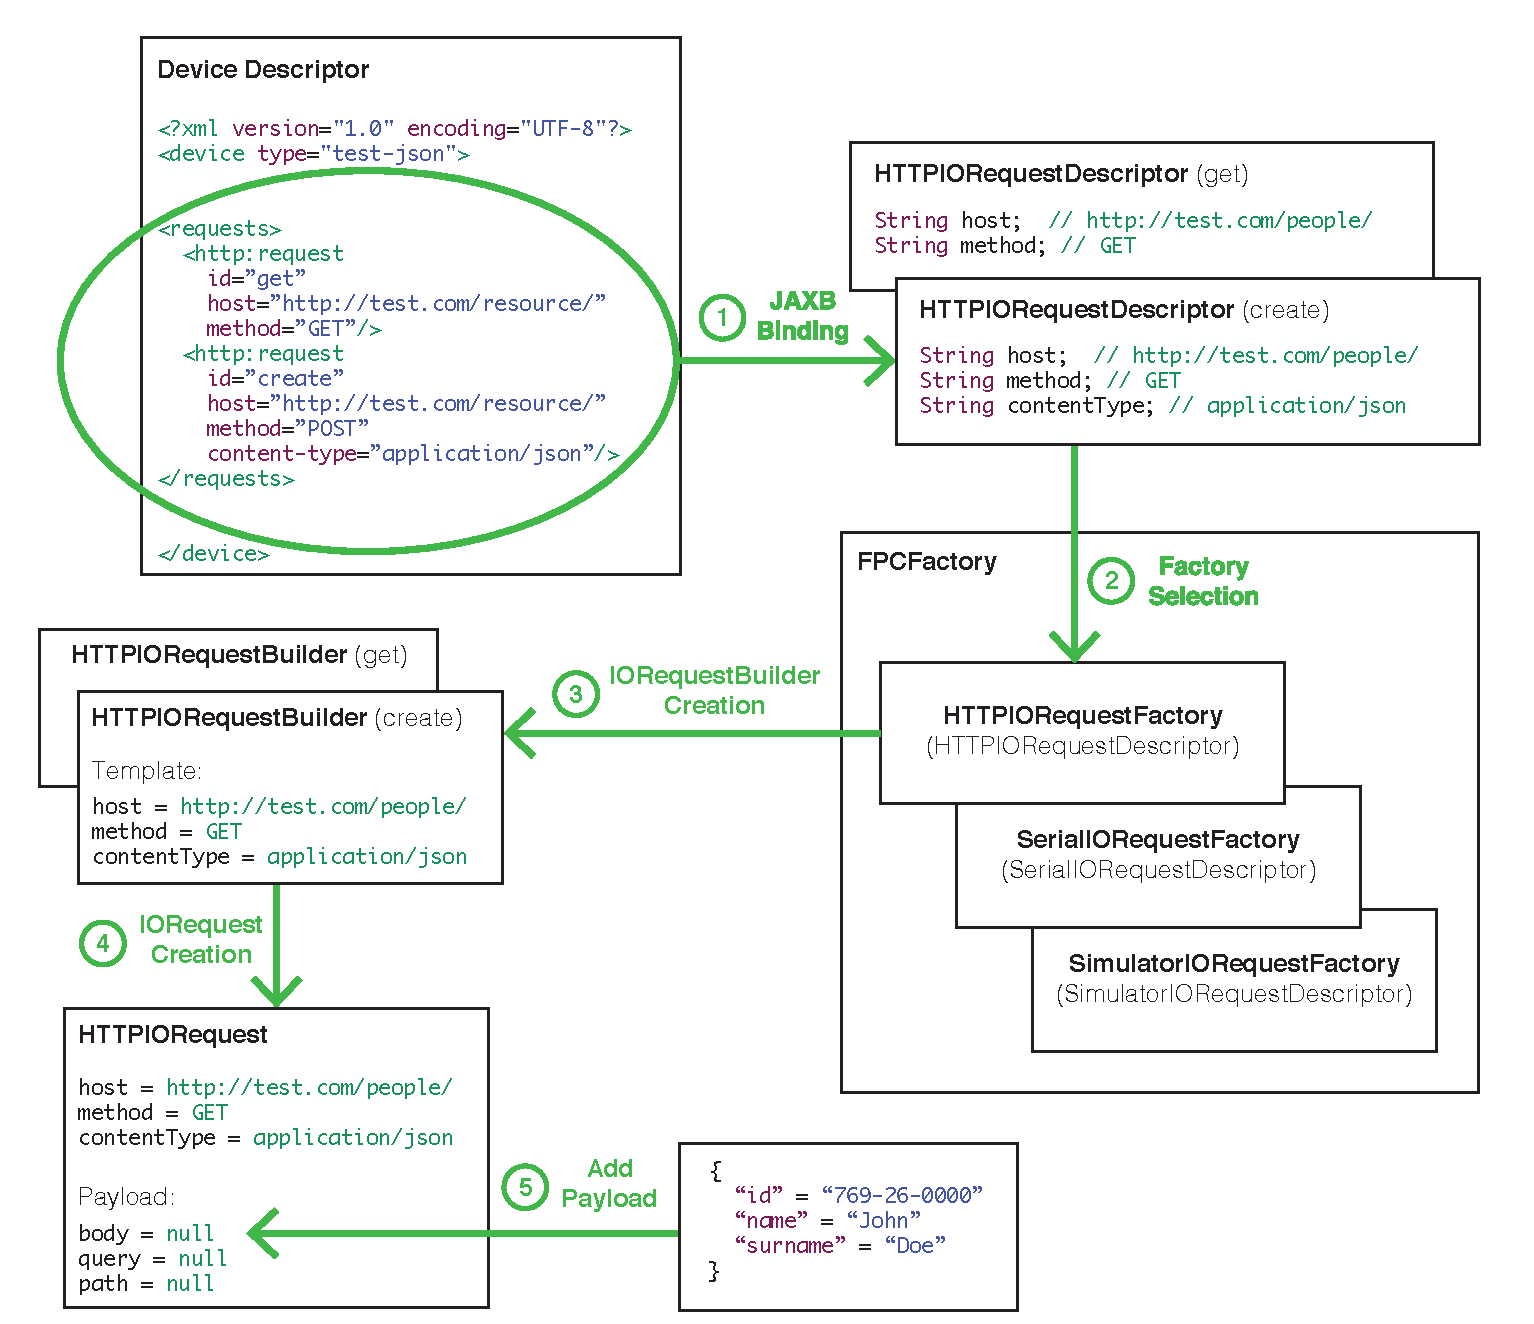
\includegraphics[width=\textwidth]{imgs/iorequest_creation_process.pdf}
\caption{The IORequest creation process}
\label{fig:iorequest.creation}
{
\begin{figurenote}
This figure illustrates the autonomous creation of \texttt{IORequest} objects.
Steps 1 to 3 are performed only once after receiving the Device Descriptor,
whereas steps 4 and 5 are repeated every time the REST API is to be invoked.
\begin{enumerate}
  \itemsep0em
  \item JAXB binds the XML Device Descriptor to an apropriate
\texttt{IORequestDescriptor} object using namespace information \item A
suitable \texttt{IORequestBuilderFactory} is selected at runtime using the
\texttt{acceptedIORequestDescriptorClass()} method
  \item The information contained in the \texttt{IORequestDescriptor} is used
to create a new \texttt{IORequestBuilder} \item The \texttt{IORequestBuilder}
is used to create new \texttt{IORequest} copies using the internal template
  \item The newly created \texttt{IORequest} objects can be populated with
\texttt{Payload} parameters as needed \end{enumerate}
\end{figurenote}
}
\end{figure}

\texttt{IORequestBuilder}s are created by means of an
\texttt{IORequestBuilderFactory}, an object that implements the now familiar
Factory design pattern. Creation proceeds as follows: the request template is
loaded from an XML Device Descriptor, bound to an appropriate
\texttt{IORequestDescriptor}, and processed by the
\texttt{IORequestBuilderFactory} to create the corresponding
\texttt{IORequestBuilder}. Similarly to what already seen in the previous
section, every \texttt{IORequestBuilderFactory} implements an
\texttt{acceptedIORequestDescriptorClass()} method, which can be used to
dynamically determine if a factory object can parse a specific type of
\texttt{IORequestDescriptor}. It should come as no surprise that every
\texttt{IORequestBuilder} class is provided with complementary
\texttt{IORequestBuilderFactory} and \texttt{IORequestDescriptor}
implementations.

\begin{figure}[!hbt]
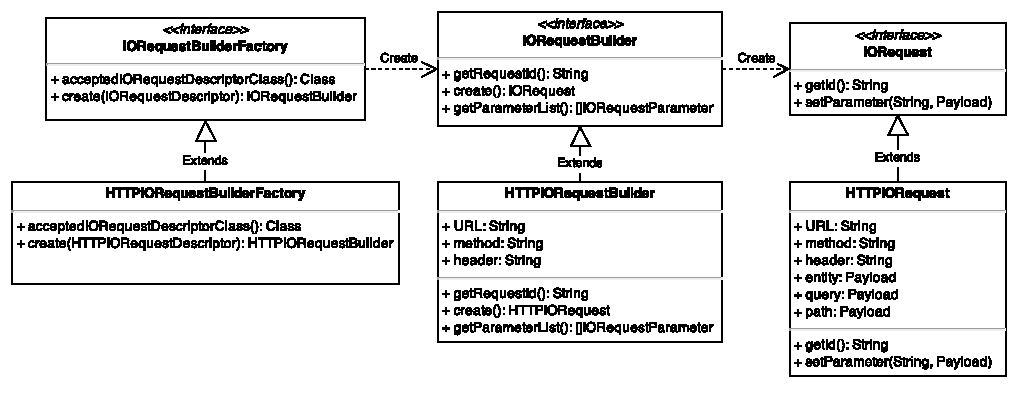
\includegraphics[width=\textwidth]{imgs/iorequest.pdf}
\caption{The extended IORequest class diagram. For additional information about
the IORequestParameter object consult listing 1.5.} \label{fig:iorequest.class}
\end{figure}


\subsection{Handling asynchronous I/O operations}

As mentioned in previous sections, communication with a device connected to the
PerLa Middleware is achieved by means of the \texttt{Channel.submit()} method.
Invocations of \texttt{submit()} are non-blocking; control flow is immediately
returned to the caller, thus allowing other computations to be performed while
the requested I/O operation is being processed.

As can be seen in listing~\ref{lst:channel}, \texttt{submit()} requires two
parameters: an \texttt{IORequest} and an \texttt{IOHandler} callback object.
The former specifies which I/O operation is to be performed, while the latter
allows the caller to be asynchronously notified of its completion.

The \texttt{IOHandler} interface is composed of two methods, namely
\texttt{complete()} and \texttt{error()}, which are invoked when processing of
an I/O operation comes to an end. It is important to note that both these
methods always carry context information in the form of an \texttt{IORequest},
which is guaranteed to be the same exact object used for starting the I/O
operation whose completion is being notified. For this reason,
\texttt{IOHandler} can be considered the nexus of the asynchronous invocation
model, as it connects \texttt{IORequest} objects with the outcome of the
corresponding I/O operation performed by the \texttt{Channel}.

\lstset{language=Java}
\begin{lstlisting}[float,floatplacement=H,caption=The IOHandler
interface,label={lst:iohandler}]
public interface IOHandler {
	public void complete(IORequest request, Optional<Payload> result);
	
	public void error(IORequest request, Throwable cause);
}
\end{lstlisting}

\lstset{language=Java}
\begin{lstlisting}[float,floatplacement=!hbt,caption=The IOTask
interface,label={lst:iotask}]
public interface IOTask {
	public void cancel();
	
	public IORequest getRequest();
	
	public boolean isCancelled();
	
	public boolean isDone();
}
\end{lstlisting}

Semantically, an invocation of the \texttt{complete()} method is always
associated with the successful termination of an I/O operation. As shown in
listing~\ref{lst:iohandler}, this method includes an optional \texttt{Payload}
object, that contains all data received from the endpoint device. A call to
\texttt{complete()} with an empty \texttt{Payload} indicates that the I/O
operation was completed without errors, but no data was received. Conversely,
an invocation of the \texttt{error()} method indicates that the I/O operation
was aborted before completion. In this case the cause of failure is always
notified through the \texttt{cause} parameter.

From the point of view the Java memory model, the \texttt{Channel.submit()}
creates a happens-before relationship with \texttt{IOHandler.complete()} and
\texttt{IOHandler.error()}, viz. any side effect generated by the code that led
to the \texttt{submit()} invocation is guaranteed to be visible in the
\texttt{complete()} and \texttt{error()} callback methods.

Asynchrous execution does not imply loss of control; ongoing I/O operations can
be monitored or cancelled by means of the \texttt{IOTask} object acquired upon
submitting an \texttt{IORequest}. Listing~\ref{lst:iotask} shows all methods of
the \texttt{IOTask} interface; method names are self explanatory, and the
reader should be able to deduce their purpose just by analyzing their 
signature. The only nuance worth mentioning is that
\texttt{isCancelled()} always implies \texttt{isDone()} (i.e., all cancelled
I/O operations are also complete), while the opposite does not hold (i.e., not
all complete I/O operations were cancelled).

\begin{figure}[!hbt]
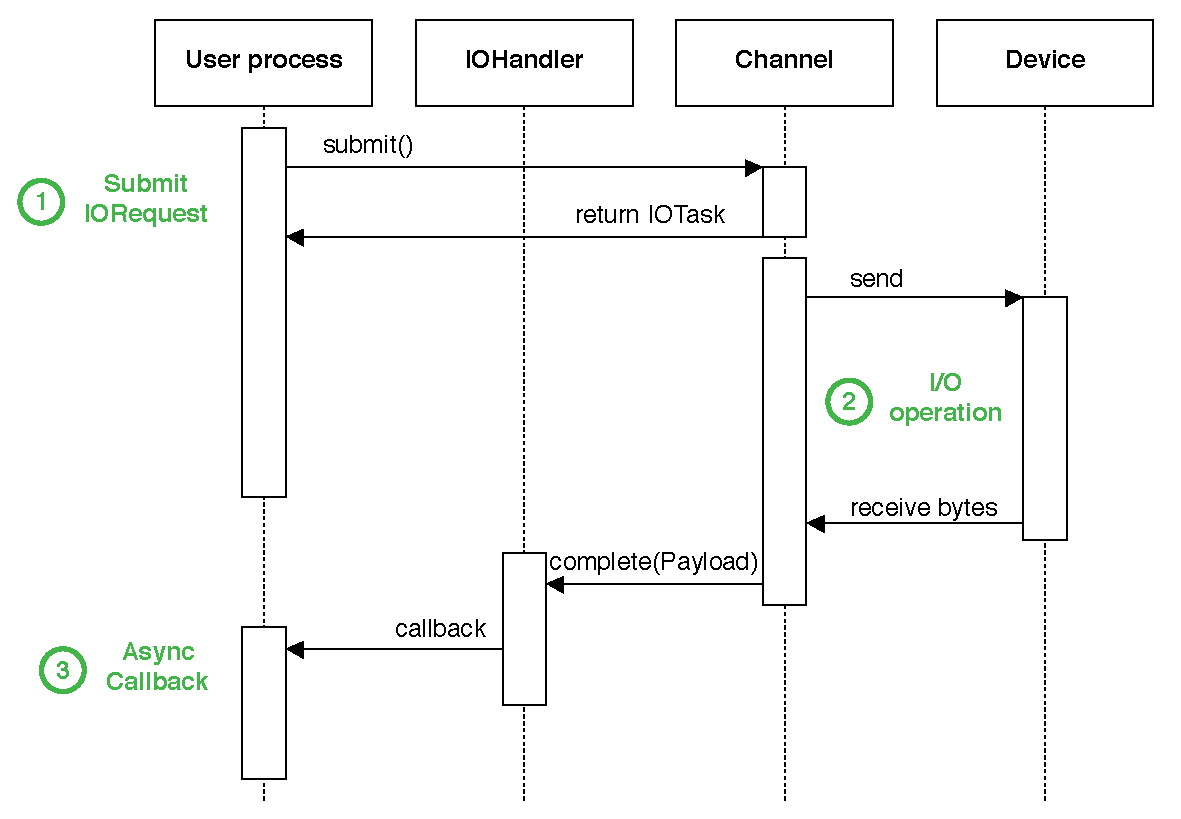
\includegraphics[width=\textwidth]{imgs/async_channel_sequence.pdf}
\caption{Sequence diagram of an asynchronous I/O operation. Note that the user
process and the I/O operation are executed in parallel.}
\label{fig:channel.async}
\end{figure}

The \texttt{Channel} interface is also designed to manage completely
asynchronous I/O operations, namely communication efforts spontaneously
initiated by the remote device. This communication model is popular among WSNs,
as it is often employed to handle periodic data streams or events happening
at irregular intervals. Such I/O operations can be handled through a catch-all
\texttt{IOHandler} set with the \texttt{setAsyncIOHandler()} method
(listing~\ref{lst:channel}). Since the communication is not initiated by the
Middleware, the \texttt{complete()} and \texttt{error()} callback methods will
be invoked with the \texttt{IORequest} parameter set to \texttt{null}.


\subsection{Implementations: HTTPChannel and SimulatorChannel}
\label{sec:channel.implementations}

Full examples of actual implementations, complete with XML descriptor snippets


\section{Handling data}
\label{sec:components.mapper}

\texttt{Payload} is a container for raw sequences of bytes. Despite its
semplicity, this class forms the foundation of the entire PerLa Middleware, as
it is the vessel that conveys all information passing through the
\texttt{Channel} interface.

The data encapsulated in a \texttt{Payload} object is accessed one byte at a
time. This granularity level is ideal for the implemention of an I/O access
layer, whose sole concern consists in the transmission of information between
two endpoints, but is not suited to other forms of data management. Processing
the information contained in a \texttt{Payload} can be unwieldy and
unnecessarily complex; the byte-oriented interface doesn't provide any facility
for leveraging the underlying structure of the enclosed data, and even a simple
action like retrieving a particular value in a complex data structure can
easily become a daunting task.


\subsection{The Message interface}

\texttt{Message}s are structured data containers that enclose a group of
individual items called fields. The chief advantage that this data structure
provides over the simpler \texttt{Payload} object consists in the possibility
of addressing information by field name, a convenient feature that dispenses
with the burden of managing data in byte-sized chunks. The methods available in
the \texttt{Message} interface are shown in listing~\ref{lst:message}.

\lstset{language=Java}
\begin{lstlisting}[float,floatplacement=!hbt,caption=The Message
interface,label={lst:message}]
public interface Message {

    public String getType();

    public boolean hasField(String name);

    public Object getField(String name)
                throws IllegalArgumentException;

    public void setField(String name, Object value)
                throws IllegalArgumentException;

    public void appendElement(String name,Object element)
                throws IllegalArgumentException;

    public boolean validate();

}
\end{lstlisting}

The specific structure of a \texttt{Message} is defined by its data type, which
can be queried through the \texttt{getType()} method. This property
unequivocally identifies the set of fields contained in a \texttt{Message} in
terms of field \textbf{name}, field \textbf{type} and field \textbf{qualifier}.

The field \textbf{name} is a textual string that uniquely identifies one
specific data item in the scope of a single \texttt{Message}. It can be used to
retrieve or set the value of a field through the \texttt{getField()} and
\texttt{setField()} methods respectively.

The \textbf{type} attribute defines the set of legal values that can be stored
in a field, together with the operations that can be performed on those values.
It is worth mentioning that field type information is used to statically verify
the type safety of nearly all data management operations performed on a
\texttt{Message} (consult section~\ref{sec:components.script} for additional
information). The following primitive data types are currently supported by the
Middleware:
\begin{itemize}
  \item \textbf{INTEGER}: a 32 bit signed two's complement integral data type
  \item \textbf{FLOAT}: a single-precision 32 bit IEEE 745 floating point
  \item \textbf{BOOLEAN}: a data type with only two values, true or false
  \item \textbf{STRING}: a string of characters with UTF-16 encoding
  \item \textbf{TIMESTAMP}: a date with timezone, currently implemented using
  Java's \textbf{ZonedDateTime} class.
  \item \textbf{ID}: a unique label that identifies a single node registered
  in the PerLa Middleware. The current implementation uses a 32 bit integer. 
\end{itemize}
Besides the six primitive data types presented above, a field can also hold a
nested \texttt{Message}. In this case, the type attribute must be set to the
particular type of \texttt{Message} that is to be stored in the field. 

The \textbf{qualifier} attribute is employed to define additional field
properties. It can be set to one of the following values:
\begin{itemize}
  \item \textbf{SIMPLE}: a normal field whose value can be set and retrieved
  using the \texttt{setField()} and \texttt{getField()} methods.
  \item \textbf{LIST}: a field that can hold multiple elements of the same
  type. New values can be added with the \texttt{appendElement()} method, while
  the entire list is retrieved through the conventional \texttt{getField()}
  method. List-qualified fields preserve the order of insertion of the
  individual elements.
  \item \textbf{STATIC}: a field whose value is statically set during
  declaration.  Any attempt to modify a statically-qualified field with either
  the \texttt{setField()} or the \texttt{appendElement()} methods will cause an
  exception to be thrown. It is important to note that static field values are
  set on a per-type basis; this means that all \texttt{Message}s of the same
  type will share the same field values for each static field (if any). 
\end{itemize}


\subsection{From Payload to Message: the Mapper interface}

\texttt{Message} objects are a convenience introduced for simplifying data
management operations in the PerLa Middleware. They provide structured access
to information, a familiar set of primitive data types, and a selection of
tools for combining basic values into complex data structures. In spite of
these advantages, the \texttt{Message} interface is a high level abstraction
that cannot be employed where a \texttt{Payload} is expected, since it doesn't
provide any method for accessing its contents as a simple sequence of bytes.
As a consequence, \texttt{Message}s can't be directly used to perform any kind
of I/O operation.

This structural gap is bridged by the \texttt{Mapper}, an interface whose
primary function consists in converting \texttt{Payload} objects into
\texttt{Message}s and vice-versa. The conversion process is designated as
\textit{marshalling} when a structured \texttt{Message} is encoded into a
\texttt{Payload}, and \textit{unmarshalling} when a byte sequence enclosed in a
\texttt{Payload} is decoded into a \texttt{Message} object. These two
operations are performed through the \texttt{marshal()} and
\texttt{unmarshal()} methods respectively (see listing~\ref{lst:mapper}).


\lstset{language=Java}
\begin{lstlisting}[float,floatplacement=!hbt,caption=The Mapper
interface,label={lst:mapper}]
public interface Mapper {

    public String getMessageType();

    public FieldDescriptor getFieldDescriptor(String name);

    public Collection<FieldDescriptor> getFieldDescriptors();

    public FpcMessage createMessage();

    public FpcMessage unmarshal(Payload payload);

    public Payload marshal(FpcMessage message);

}
\end{lstlisting}

Every \texttt{Mapper} implementation is designed to support a specific data
format. The \texttt{JSONMapper}, for example, handles JSON-formatted byte
streams, whereas the \texttt{URLEncodedMapper} specializes in the conversion of
URL-encoded HTTP entities. The additional decoupling provided by the
\texttt{Mapper} interface builds over the pluggable \texttt{Channel} design,
thus allowing \texttt{Mapper}s and \texttt{Channel}s to be selected
independently of each other. This separation of concerns allows the same
\texttt{Channel} to be used in conjunction with multiple \texttt{Mapper}s to
distribute information using different data formats, as shown in
figure~\ref{fig:mapper_channel}.

\begin{figure}[h!]
    \centering
    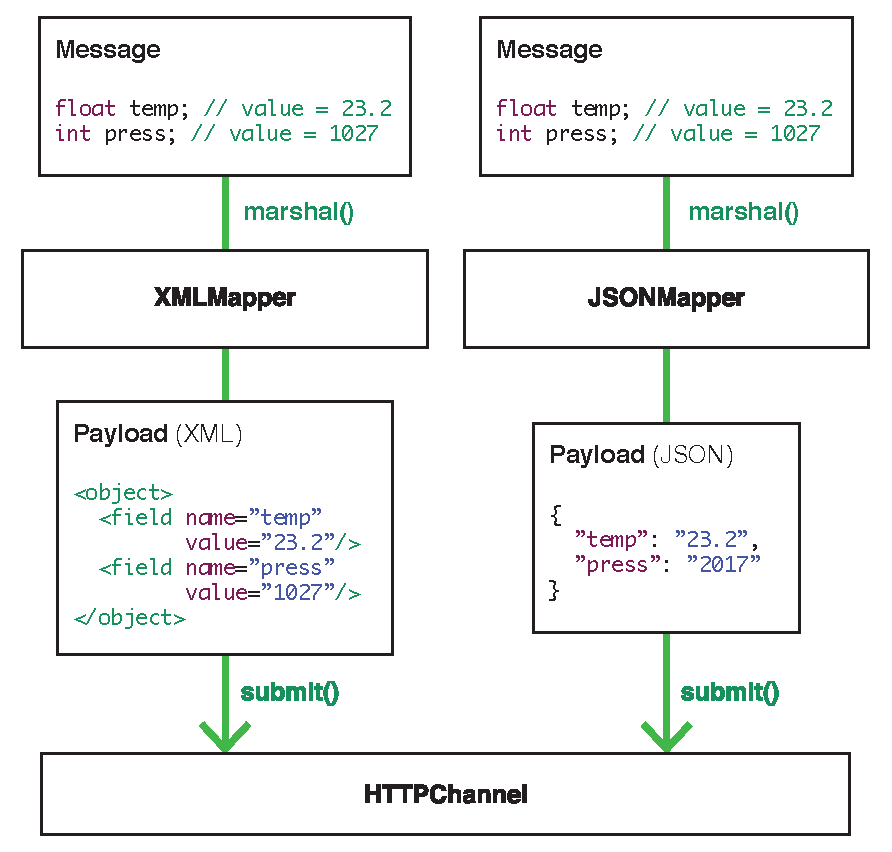
\includegraphics[scale=0.8]{imgs/mapper_channel.pdf}
    \caption{Using a single \texttt{Channel} to transmit data marshalled with
    different \texttt{Mapper}s}
    \label{fig:mapper_channel}
\end{figure}

The \texttt{Mapper} interface is one of the extension points that final users
can utilize to expand the core functionalities of the PerLa Middleware. New
\texttt{Mapper} implementation can be added to support new data formats or 

Different \texttt{Mapper} implementations may be provided to support 

The additional level of decoupling provided by the \texttt{Mapper} interface is
used to 

Prior to transmission, \texttt{Message}s are marshalled into a suitable
\texttt{Payload}

The PerLa Middleware exploits this additional level of decoupling to support
all provide support for different data formats. the different data formats found in a Pervasive System.



Data exchanged between the
Middleware and an endpoint device may be structured using a plethora of
formats, like JSON and XML (REST APIs), C-like data structures (low-power or
embedded node), serialized Java classes (Java RMI APIs), proprietary data
encoding mechanism, and many more. The \texttt{Mapper} interface allows 

This
diversity is a characteristic trait of Pervasive Network environments, and the
\texttt{Mapper} interface is the component 

not only support different formats, but different formats coexist in a
pervasive network

a single mapper would effectively limit the class of devices with which the PerLa
middleware is able to manage




The \texttt{Mapper}
interface thus introduces an additional level of indirection that is
fundamental for the management of different data encoding schemes.

The additional level of decoupling introduced with the \texttt{Mapper}
interface is fundamental design feature that Data transmitted between the middleware and
an endpoint device may be organized using different 

The additional level of decoupling introduced with the \texttt{Mapper}
interface is a fundamental design choice that allows the PerLa Middleware to
support different encoding schemes. Data transmitted between the middleware and
an endpoint device may be organized using different 

this allows the same channel to be used for transmitting data encoding usind
different techniques

decoupling

The gap between \texttt{Payload}s and \texttt{Message}s is bridged with the
\texttt{Mapper} interface. \texttt{Mapper}s 


which is still
required to perform any kind of I/O operation. The \texttt{Mapper} interface is required to bridge this
gap.

The \texttt{Message} interface is however a high level abstraction that cannot
be employed as a direct substitute for a \texttt{Payload} object, which is still
required to perform any kind of I/O operation. The \texttt{Mapper} interface is required to bridge this
gap.

Mappers are responsible for instatiating, marshalling and unmarshalling
messages

\subsection{Declaring new Message types}


Character encoding may depends on the message, not the single field

information agnostic

A set of bytes is usually encoded from a message

Difference between unstructured collections of bytes and a Message.
Message structures field types and accessor methods to retrieve and set field
data. Working with composite fields and vector fields (append)

Managing messages with the Mapper: create new message, discover message
fields at runtime, marshal and unmarshal operations

Creating new messages: the MapperFactory interface and the relationship with
the XML


Using the validate() method to manage multiple message types



\subsection{Handling composite data structures}

\subsection{Managing multiple message types}

\subsection{Implementations: JSONMapper and URLEncodedMapper}


\section{Data management: Scripts}
\label{sec:components.script}

\subsection{From Messages to Records}

\subsection{Available instructions}

\subsection{Engine architecture and execution model}

\subsection{Script examples}


\section{Putting it all together: the FPC}

\subsection{Data access interface}

\subsection{Controlling the remote device}

\subsection{Scheduling mechanism}


\section{Device Descriptor and FPC Factory}

\subsection{The XML Device Descriptor}

\subsection{FPC Factory}

\subsection{Registry}

\subsection{Complete XML Device Descriptor examples}
